\section{Introduction}

%===========================================================================================
% Motivation
%===========================================================================================
After intelligence with reinforcement learning beat humans \citep{tesauro1995temporal,mnih2015human,silver2016mastering}, reinforcement learning has been expected to be applied into industry such as stock trade, autonomous cars, smart grid and IoT. 
In a world which realized the industrial application in the future, various types of companies will own their agents to improve their revenue.
The situation can be regarded as one that each agent are independently solving problems of partially observed Markov decision process (POMDP).

These agents in the companies are designed to maximize their own reward independently of each other. 
However, if the agents could exchange their own information, the entire revenue of the stakeholders would further increase.
As each agent has limited visibility of the environment, exchanging information among the agent will be helpful to solve their own tasks.
Thus, this paper aims to realize a society in which stakeholders which can have a conflict of interest trade their own information.
%Imagine diamond production with social division by different companies from raw material collection, processing to selling.
%If we can realize representation learning in the each layers as the social division, a single company can yield revenue more than one by itself. 

%in the case the company does it by itself.
%If the agents exchange their own information each other, entire revenue will be improved more than individuals.
%These agents in the companies are closed to maximize their own reward.
%Using economic metaphor, similarly to a supply chain of diamond from a company which collects raw material, one which processes it to one which sells it.
%Although agents in the companies are closed to maximize their own reward, if the agents exchange their own information each other, entire revenue will be improved more than individuals.

We regard the situation as communication in multi-agent reinforcement learning (MARL), addressed by several existing methods such as R/DIAL \citep{foerster2016learning} and CommNet \citep{sukhbaatar2016learning}.
CommNet is a state-of-the-art of MARL which considers communication among agents, 
and the feature is learning among agents with backpropagation.

In the case when we are trying to consider MARL in which different stakeholders make different agents which communicate each other, it needs design of incentive distribution (e.g., monetary payment) and a framework without {\em trusted third party} (TTP).
TTP \citep{wu1999game,sandholm2002possibility} is a neutral administrator which assumes distribution of reward for all the participants, supposed implicitly by most of existing literatures with regard to MARL \citep{agogino2006quicr,sukhbaatar2016learning,foerster2016learning,foerster2017counterfactual}.
While TTP is required to be neutral against all the participants,
several configuration of peer-to-peer trade such as inter-industry and -country trade cannot prepare TTP.
If untrusted third party assumes reward distribution, it can undesirably make reward for partial participants higher than necessity.

To the best of our knowledge, no existing literatures discuss the reward distribution on the configuration above.
Since CommNet assumes an environment which distributes a uniform reward to all the agents, 
in the case distributing limited reward in supply such as money, it causes {\em Tragedy of the Commons} \citep{lloyd1833two} in which contributing agents' reward will reduce due to participant of free riders.
Although there are several MARL methods which distributes reward depends on their contribution such as QUICR \citep{agogino2006quicr} and COMA \citep{sukhbaatar2016learning}, they suppose the existence of TTP, and hence it cannot be applied into our situation.

%===========================================================================================
% Objective
%===========================================================================================

Our proposed method, {\em Neuron as an Agent} (NaaA) extends CommNet to realize incentive distribution
in MARL without TTP with two key ideas: (i) inter-agent reward distribution and (ii) auction theory.
The reason why we introduce auction theory is inter-agent reward distribution is insufficient for optimization.
An agent in NaaA maximizes {\em profit}, difference between reward which it receives and cost which it redistributes to other agents.
If we optimize the framework naively, we obtain a trivial solution that agents make their cost zero to maximize the profit.
Then, NaaA employs game design with auction theory to keep cost being smaller than necessity.
As a theoretical result, we show that an agent autonomously evaluates {\em counterfactual return} as other agent's value.
Counterfactual return equals to discounted cumulative sum of counterfactual reward \citep{agogino2006quicr} which QUICR and COMA distribute.
NaaA realizes reward distribution which make it pareto improvement more than inter-agent reward distribution.

\begin{figure*}[tb]
	\centering
	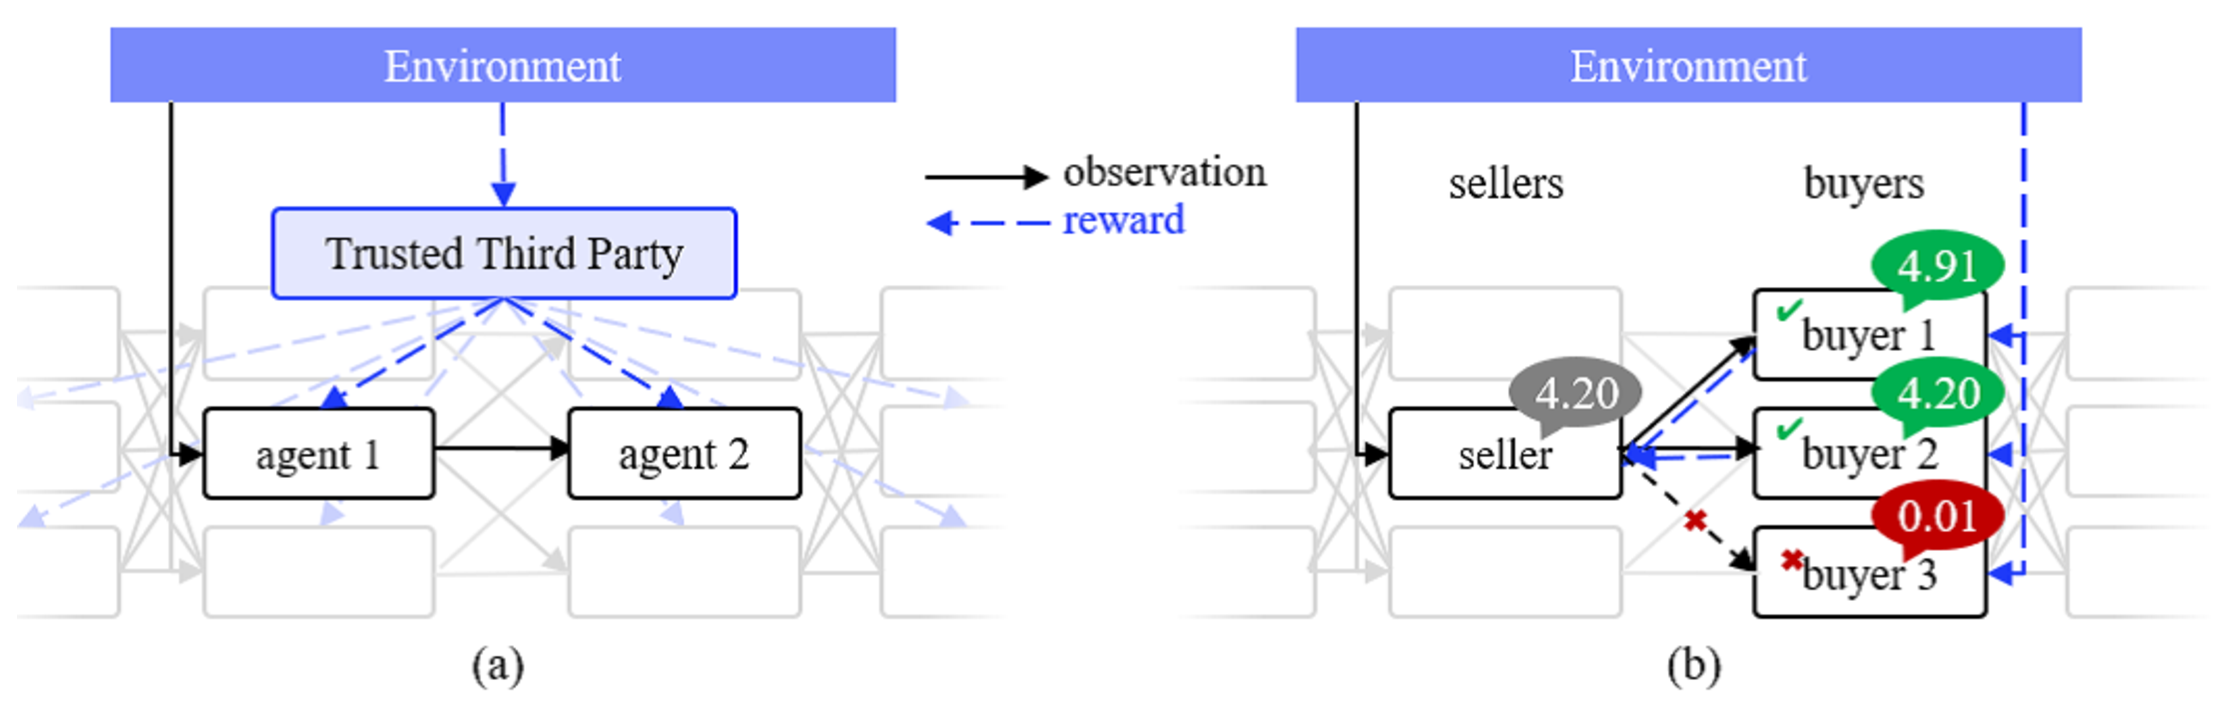
\includegraphics[width=\linewidth]{img/TTP.eps}
	\caption{
		A schematic illustration of reward disteribution models in MARL.
		{\bf (a)} Centralized reward distribution model \citep{agogino2006quicr,sukhbaatar2016learning,foerster2016learning,foerster2017counterfactual}
		{\bf (b)} Inter-agent reward distribution model (our model). Some agents receive reward from the environment directly,  
			and redistribute to other agents. The agents maximize their profit instead of reward.
		{\bf (c)} Neuron as an Agent (NaaA). Inter-agent reward distribution includes reward backpropagation along the connections. 
	}
	\label{fig:ttp}
\end{figure*}

NaaA enables us to trade of representation in peer-to-peer and regard a unit in a neural network as an agent ultimately.
As NaaA can regard a unit as an agent without loss of generality indeed, this paper uses the setting.
We illustrate the concept proposed method in \figurename~\ref{fig:ttp}.

In the experiment, we use an environment which extends ViZDoom \citep{kempka2016vizdoom}, a POMDP environemnt, to MARL.
We put two agents in the environment.
The one is a cameraman who send information, and the another one is a main player to defeat enemies with a gun.
We confirm that the cameraman learns cooperative action to send information in dead angle, behind of main player, and outperform CommNet in score.

Interestingly, NaaA can apply to a single-agent as well as multi-agent setting since it learns optimal topology between the units. %with respect to supervised learning
As a further application, we propose {\em Adaptive DropConnect} (ADC), which combines DropConnect \citep{wan2013regularization}, which randomly masks the topology, with an adaptive algorithm, which prunes connections with less counterfactual return with higher probability.
Experimental result in classification and reinforcement learning task shows ADC outperforms DropConnect.
%Subsequently, we present that our trading model leads the model to learning optimal topology between the units with respect to supervised learning as well as MARL.
%It uses $\varepsilon$-greedy as an exploration policy, and is equivalent to DropConnect in the case of $\varepsilon = 1$. It is equivalent to counterfactual return maximization, which constructs the topology deterministically in the case of $\varepsilon = 0$.

% Organization
The remaining part of this paper is organized as follows. 
First, we describe the two key ideas: inter-agent reward distribution and auction theory. 
After introducing related works, we show the experimental result in ViZDoom.
Next, we show ADC and its experimental result as a further application. 
Then, we conclude this paper.
